\documentclass{llncs}
\usepackage[utf8]{inputenc}
\usepackage[T1]{fontenc}
\usepackage{makeidx}  % allows for indexgeneration
\usepackage{graphicx}
\usepackage[english]{babel}
\usepackage{float}
\usepackage{wrapfig}
\usepackage{textcomp}
\usepackage{hyperref}
\usepackage[multiple]{footmisc}
\usepackage{acronym}
\tolerance=1000

\urldef{\mailsa}\path|{joel.kuiper, m.a.swertz}@rug.nl|
\urldef{\mailsb}\path|iain.marshall@kcl.ac.uk|
\urldef{\mailsc}\path|byron.wallace@utexas.edu|

\acrodef{ebm}[EBM]{Evidence-based Medicine}
\acrodef{ml}[ML]{machine learning}
\acrodef{pdf}[PDF]{Portable Document Format}
\acrodef{cdsr}[CDSR]{Cochrane Database of Systematic Reviews}
\acrodef{svm}[SVM]{Support Vector Machine}

\institute{
  University of Groningen P.O. Box 30001, 9700 RB Groningen \\ \mailsa
  \and King's College London, London SE1 3QD, UK \\ \mailsb
  \and University of Texas at Austin, Austin, TX 78712, USA \\ \mailsc}

\begin{document}
\setcounter{tocdepth}{3}

%% Autogenerated, do not edit
\newcommand{\revisiondate}{2014-04-24}
<<<<<<< HEAD
\newcommand{\revision}{3f2c73a}
=======
\newcommand{\revision}{d58899a}
>>>>>>> 1b257ee... updates

\author{Kuiper, J\inst{1}. \and Marshall, I.J.\inst{2} \and Wallace, B.C.\inst{3} \and Swertz, M.A.\inst{1}}
%\date{\texttt{revision: \revision, date: \revisiondate}}
\title{Spá: a web-based viewer for text mining in Evidence Based Medicine}

\maketitle
\begin{abstract}
Summarizing the evidence about medical interventions is an immense undertaking, in part because unstructured \ac{pdf} documents remain the main vehicle for disseminating scientific findings.
Clinicians and researchers must therefore manually extract and synthesise information from these \acp{pdf}.
We introduce Spá,\footnote{From the Old Norse word spá or spæ referring to prophesying (prophecy)}\footnote{Source code available under GPLv3 at \url{https://github.com/joelkuiper/spa} \cite{Kuiper2014}; demo available at \url{http://spa.clinici.co/}} a web-based viewer that enables automated annotation and summarisation of \acp{pdf} via \acl{ml}.
To illustrate its functionality, we use Spá to semi-automate the assessment of bias in clinical trials.
Spá has a modular architecture, therefore the tool may be widely useful in other domains with a \ac{pdf}-based literature, including law, physics, and biology.

\end{abstract}

\acresetall
\acused{pdf}

\section{Introduction}
\label{section:intro}

Imposing structure on full-text documents is an important and practical task in natural language processing and machine learning.
\emph{Systematic reviews} are an instructive example.
Such reviews aim to answer clinical questions by providing an exhaustive synthesis of all the current evidence in published literature.
They are fundamental tools in \ac{ebm} \cite{Sackett1996,Valkenhoef2012}.
Data must be manually extracted from the literature to produce the systematic reviews.
These extraction tasks are extremely laborious, but could potentially be assisted by machine learning approaches.

As an example we consider risk of bias assessment.
Here reviewers assess, e.g., whether study participants and personnel were properly blinded \cite{Higgins2011}.
Assessing risk of bias is a time-consuming task.
A single trial typically takes a domain expert ten minutes \cite{Hartling2011}, and a single review typically includes several dozen trials.
Making matters worse, due to low rates of reviewer agreement it is regarded as best practice to have each study assessed twice by independent reviewers who later come to a consensus \cite{Hartling2009}.

Machine learning methods could provide the machinery to automate such extractions; as they can effectively impose the desired structure onto \acp{pdf}.
But if such technologies are to be practically useful, we need tools that visualize these model predictions and annotations.
Here we describe Spá, which aspires to realize this aim.

Spá is an open-source, web-based tool that can incorporate machine learning to automatically annotate \ac{pdf} articles.
As a practical demonstration of this technology, we have built a machine learning system that automatically annotates \acp{pdf} to aid \ac{ebm}.
This tool is unique in that it leverages state-of-the-art \ac{ml} models applied to full-text articles to assist practitioners of \ac{ebm}.

\begin{figure}[htb]
\vspace{-1em}
\centering
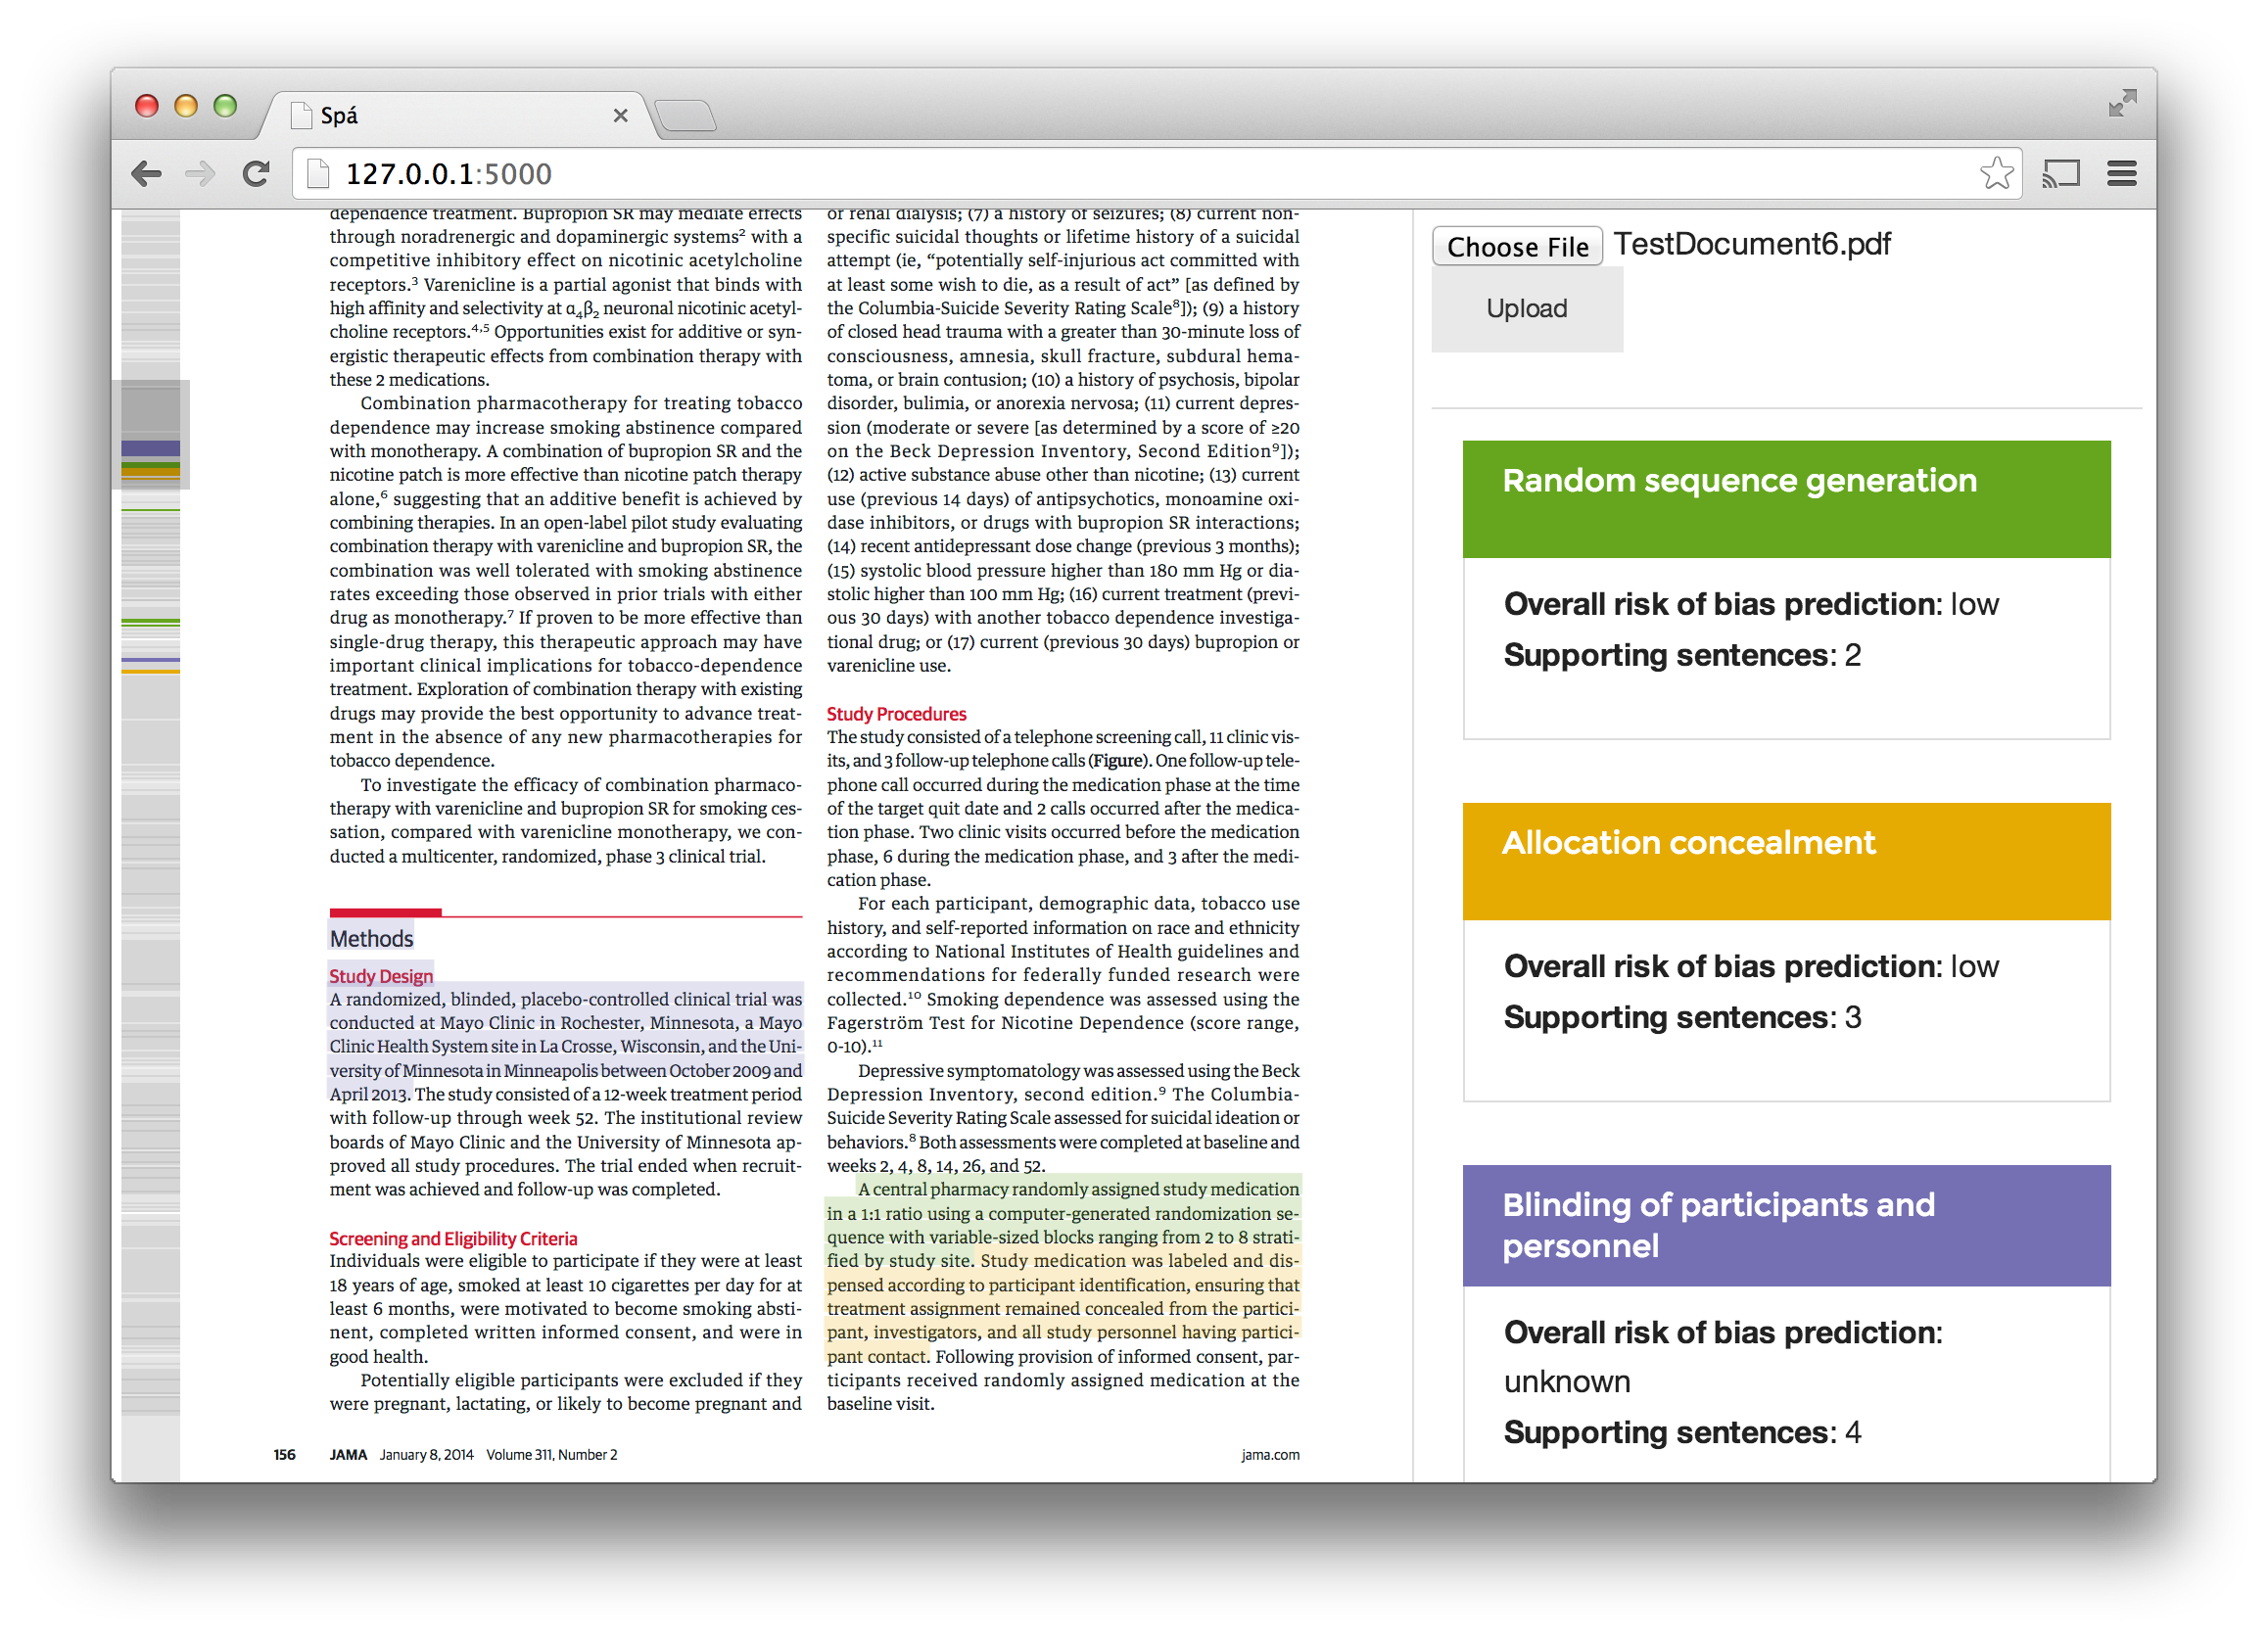
\includegraphics[width=1.0\linewidth]{./images/screenshot2.png}
\vspace{-1em}
\caption{\label{fig:screenshot}Screenshot of a \ac{pdf} with highlighted risk of bias. Here the risk of bias is assessed to be low, for example, and one of the supporting sentences for this assessment describes the randomization procedure (highlighted in green).}
\vspace{-1.5em}
\end{figure}

While our application of interest is \ac{ebm}, we emphasize that the visualization tool can be used for any domain in which one wants to annotate \acp{pdf}, e.g. genome-wide association studies or jurisprudence.
Thus the contribution of this work is two-fold, as we present:
(1) a practical tool that incorporates machine learning to help researchers rapidly assess the risk of biases in published biomedical articles, and,
(2) a general open-source system for visualizing the predictions of trained models from full-text articles on the web.

\section{Case study: Risk of Bias in \acl{ebm}}
\label{section:EBM-ML}

\subsection{Machine Learning Approaches}
To automatically assess the study risk of bias, we have leveraged the \ac{cdsr} in lieu of manually annotated data, which would be expensive to collect.
The \ac{cdsr} contains descriptions and data about clinical trials reported in existing systematic reviews.
We match the full-texts of studies to entries in the \ac{cdsr}, which contains risk of bias assessment; providing document level labels.
The \ac{cdsr} also contains quotations that reviewers indicated as supporting their assessments.
We match these strings to substrings in the \acp{pdf} to provide sentence-level supervision.
This can be viewed as a \emph{distantly supervised} \cite{Mintz09,Nguyen11} approach.

From a \ac{ml} vantage, we have two tasks for a given article: (1) predict the overall risk of bias for each of the domains, and (2) extract the sentences that support these assessments.
For both tasks we leverage standard bag-of-words text encoding and linear-kernel \aclp{svm}.
Because the risk of bias predictions are correlated across domains, we take a \emph{multi-task} \cite{Evgeniou2004} approach to classification and jointly learn a model for the domains.
We accomplish this by way of a feature space construction that includes both shared and domain-specific terms, similar to the domain adaptation approach in \cite{Daume2007}.
Specifically, we first make sentence level prediction, and then insert features representing the tokens in the predicted sentences for exploitation by the document level classifier.
Figure \ref{fig:screenshot} shows the system in use.

\section{Spá Architecture Overview}

%label{section:architecture}
%begin{wrapfigure}{}{0.5\textwidth}
% \vspace{-2em}
% 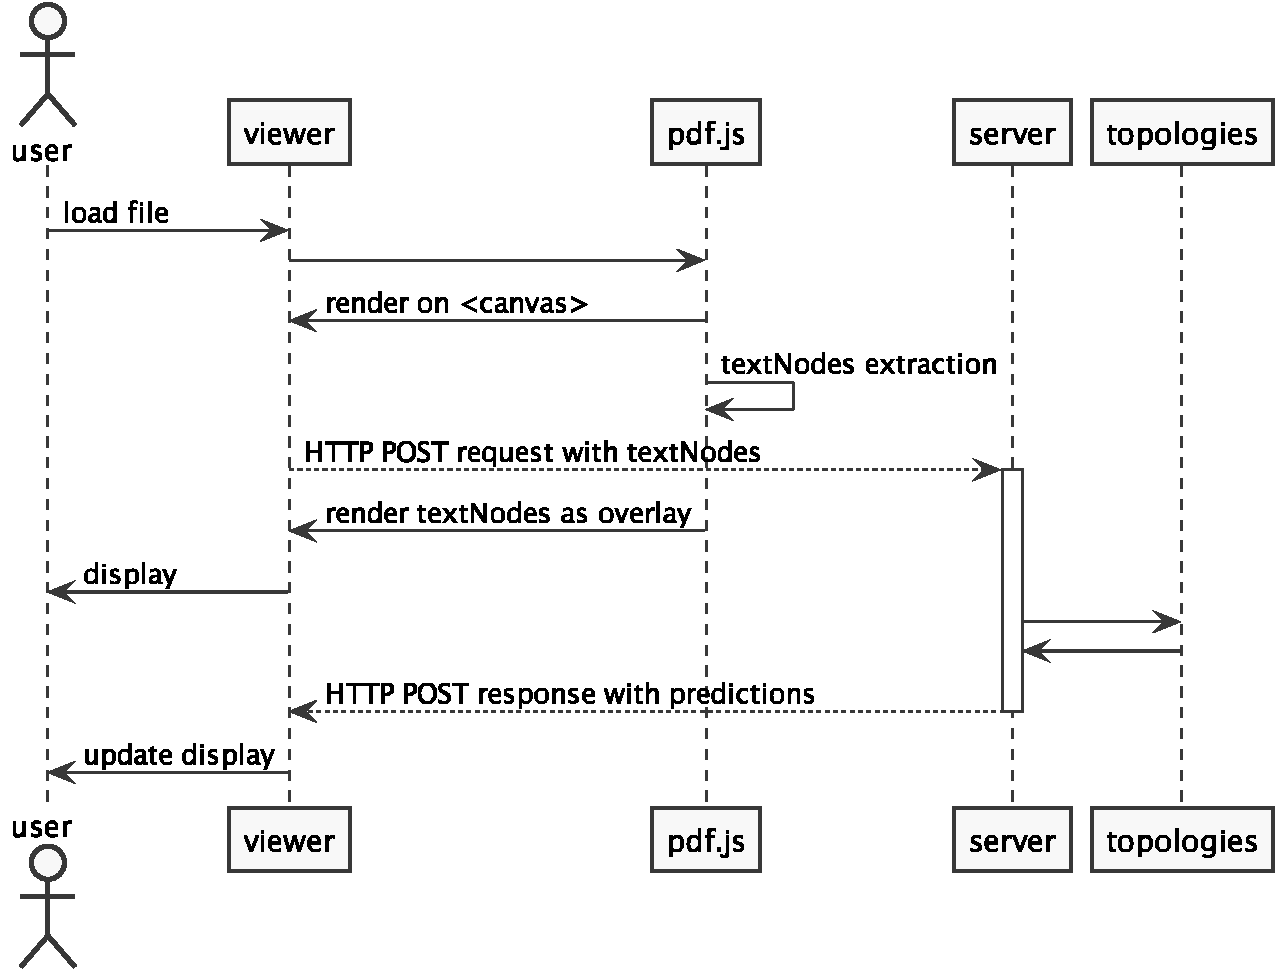
\includegraphics[width=0.6\textwidth]{./diagrams/sequence.pdf}
% \vspace{-1em}
% \caption{\label{fig:sequence}Sequence diagram of a typical request-response in Spá.}
% \vspace{-1.0em}
%end{wrapfigure}

Spá relies on Mozilla pdf.js\footnote{\url{http://mozilla.github.io/pdf.js}} for visualization of the document and text extraction.
The results of the text extraction are processed server-side by a variety of processing topologies.
Results are communicated back to the browser and displayed using React components.\footnote{\url{http://facebook.github.io/react}}

For each of the annotations the relevant nodes in the document are highlighted.
A custom scrollbar, inspired by \href{http://substance.io/}{substance.io}, that acts as a `mini-map' is projected to show where annotations reside within the document.
The user can interactively activate and inspect specific results.

\section{Future work}
We have presented a web-based tool for visualization of annotations and marginalia for \ac{pdf} documents.
Furthermore, we have demonstrated the use of this system within the context of \acl{ebm} by automatically extracting potential risks of bias.

We believe the tool to be potentially useful for a much wider range of \acl{ml} applications.
Currently we are developing a pluggable system for processing topologies, allowing developers to quickly plug in new systems for automated \ac{pdf} annotation.
Furthermore, we are working to allow users to persist annotations and marginalia, possibly embedded within the document itself, for sharing and off-line use.
The vision is to have an extensible system for machine assisted data extraction that will greatly increase both the quality and the reproducibility (i.e. data provenance) of current \acl{ebm}.

\subsubsection{Acknowledgments}
Part of this research was funded by the European Union Seventh Framework Programme (FP7/2007-2013) under grant agreement n° 261433.

\bibliographystyle{splncs}
\bibliography{references}
\end{document}
